\chapter{Design}

For bedre at forstå designet omkring spillet har vi ud fra use case 1 (Tabel \ref{usecase:1}) lavet et klassediagram som beskriver de elementer spillet består af. Det ses der, at spillet kommer til at bestå af terningerne og spillere. På figur \ref{fig:klassediagram} ses klassediagrammet. 

\section{Klassediagram}

\begin{figure}[h]
    \begin{center}
        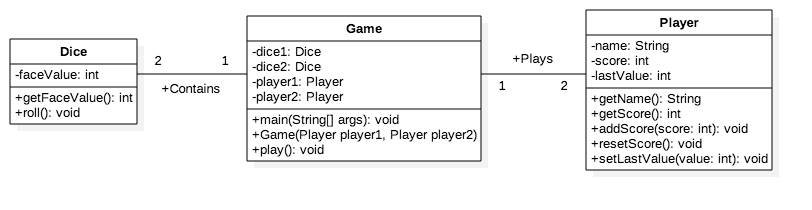
\includegraphics[width=15cm]{graphics/Klassediagram}
        \caption{Klassediagram over spillet}
        \label{fig:klassediagram}
    \end{center}
\end{figure}